\chapter{Equations Différentielles Non Linéaires}


\setlength{\parindent}{0pt}
\renewcommand{\labelitemi}{\textbullet} % Utiliser des points noirs (•)

% ==================================================================================================================================
% Cauchy-Lipschitz

\section{Cauchy-Lipschitz}

\textbf{Problème : } On cherche une condition suffisante d'existence et d'unicité d'une solution maximale au problème 
de Cauchy: 
    \[ (P) : 
        \begin{cases}
            (E) : y'(t) = f(t,y) \\ 
            (C) : y(t_0) = y_0 
        \end{cases}
    \] 

\begin{definition}[Fonction Localement Lipschitzienne]
    Soit 
        \[ f : 
            \begin{cases}
                \Omega = I \times \Omega' \longrightarrow \K^n \\ 
                (t,x) \longmapsto f(t,x)
            \end{cases} \] 
    On dit que $f$ est LLVE (localement lipschitzienne en la variable d'état i.e $x$) \underline{si} :
        \[ \forall (t_0, y_0) \in I \times \Omega', \exists [t_0 - \alpha, t_0 + \alpha] \times B_f(y_0,r) \] 
    Tel que : 
        \[ \exists k \in \R_+, \forall t \in [t_0 - \alpha, t_0 + \alpha], \text{ on a : } \] 
        \[ \boxed{ \forall x,x' \in B_f(y_0,r), \| f(t,x) = f(t,x') \| \leqslant k \| x - x'\| } \] 
    
    \emph{On cherche donc un cylindre $[t_0 - \alpha, t_0 + \alpha] \times B_f(y_0,r) \subset I \times \Omega'$ sur lequel 
    $f$ soit lipschitzienne.}
\end{definition}

\begin{comment}
    \begin{center}
        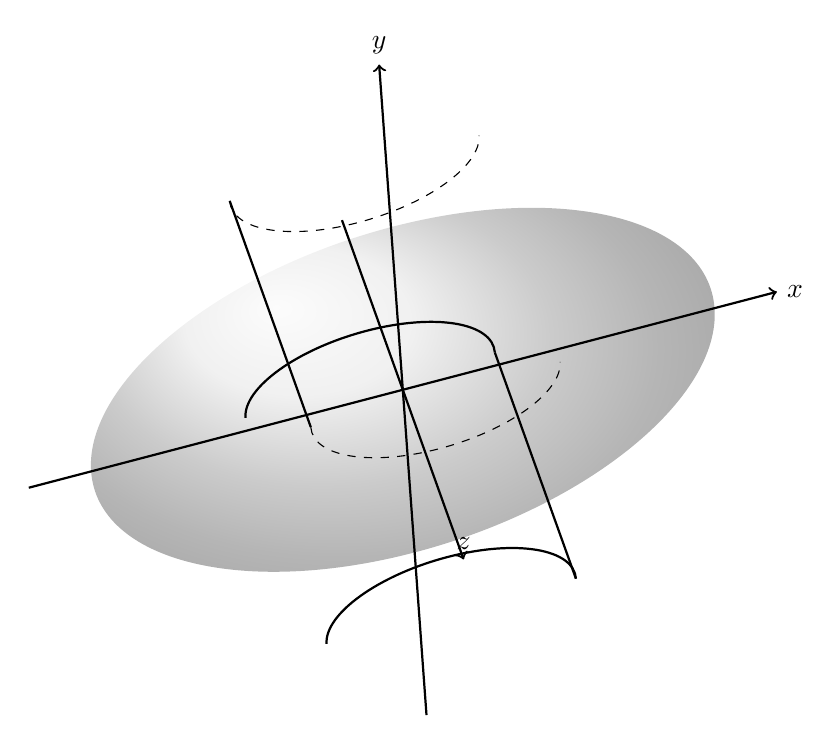
\begin{tikzpicture}
    
            % Définition de la perspective
            \begin{scope}[scale=1.5, rotate around x=10, rotate around y=30]
        
                % Boule irrégulière (ellipsoïde en 3D)
                \shade[ball color=gray!30, opacity=0.5] (0,0,0) ellipse (2.5 and 1.5);
        
                % Cylindre : bases et côtés
                \draw[thick] (1,-1,-2) -- (1,-1,2);
                \draw[thick] (-1,1,-2) -- (-1,1,2);
                
                % Dessin des bases du cylindre
                \draw[thick] (1,-1,2) arc[start angle=0, end angle=180, x radius=1, y radius=0.5];
                \draw[dashed] (-1,1,2) arc[start angle=180, end angle=360, x radius=1, y radius=0.5];
                
                \draw[thick] (1,-1,-2) arc[start angle=0, end angle=180, x radius=1, y radius=0.5];
                \draw[dashed] (-1,1,-2) arc[start angle=180, end angle=360, x radius=1, y radius=0.5];
        
                % Axes orthonormés
                \draw[thick,->] (-3,0,0) -- (3,0,0) node[right] {$x$};
                \draw[thick,->] (0,-3,0) -- (0,3,0) node[above] {$y$};
                \draw[thick,->] (0,0,-3) -- (0,0,3) node[above] {$z$};
        
            \end{scope}
        
        \end{tikzpicture}
    \end{center}
\end{comment}






